\documentclass[main.tex]{subfiles}

\begin{document}
\sloppy


\vspace{1.0cm}

\section{Design di una pipeline di rendering}\label{sec:RenderingPipeline}
Come spiegato nel capitolo \ref{subsec:1_tirocinio} dopo un primo periodo per familiarizzare con la codebase, è stato semplice intuire come, in quello stato, fosse impossibile la facile aggiunta di nuove features. Inoltre tra le TODO trovate all'interno del progetto lasciate dal tirocinante precedente, ne troviamo una che indica come vada ancora aggiunto il supporto a più ruote dello stesso tipo (Particolarità presente in molte fixture). In questo capitolo mostriamo la vecchia implementazione, gettiamo delle idee su come ricrearla in maniera più modulare e mostriamo alla fine il codice finale.

\subsection{Analisi della vecchia implementazione}\label{subsec:2_oldImplementation}
All'interno del plugin troviamo 3 materiali che si occupano del rendering della luce emessa da una fixture.
\subsubsection{Beam}\label{subsec:2_1_beam}
Questo materiale si occupa del rendering del fascio di luce visibile in aria, chiamato anche \say{beam di una fixture}.
\begin{figure}[H]
    \centering
    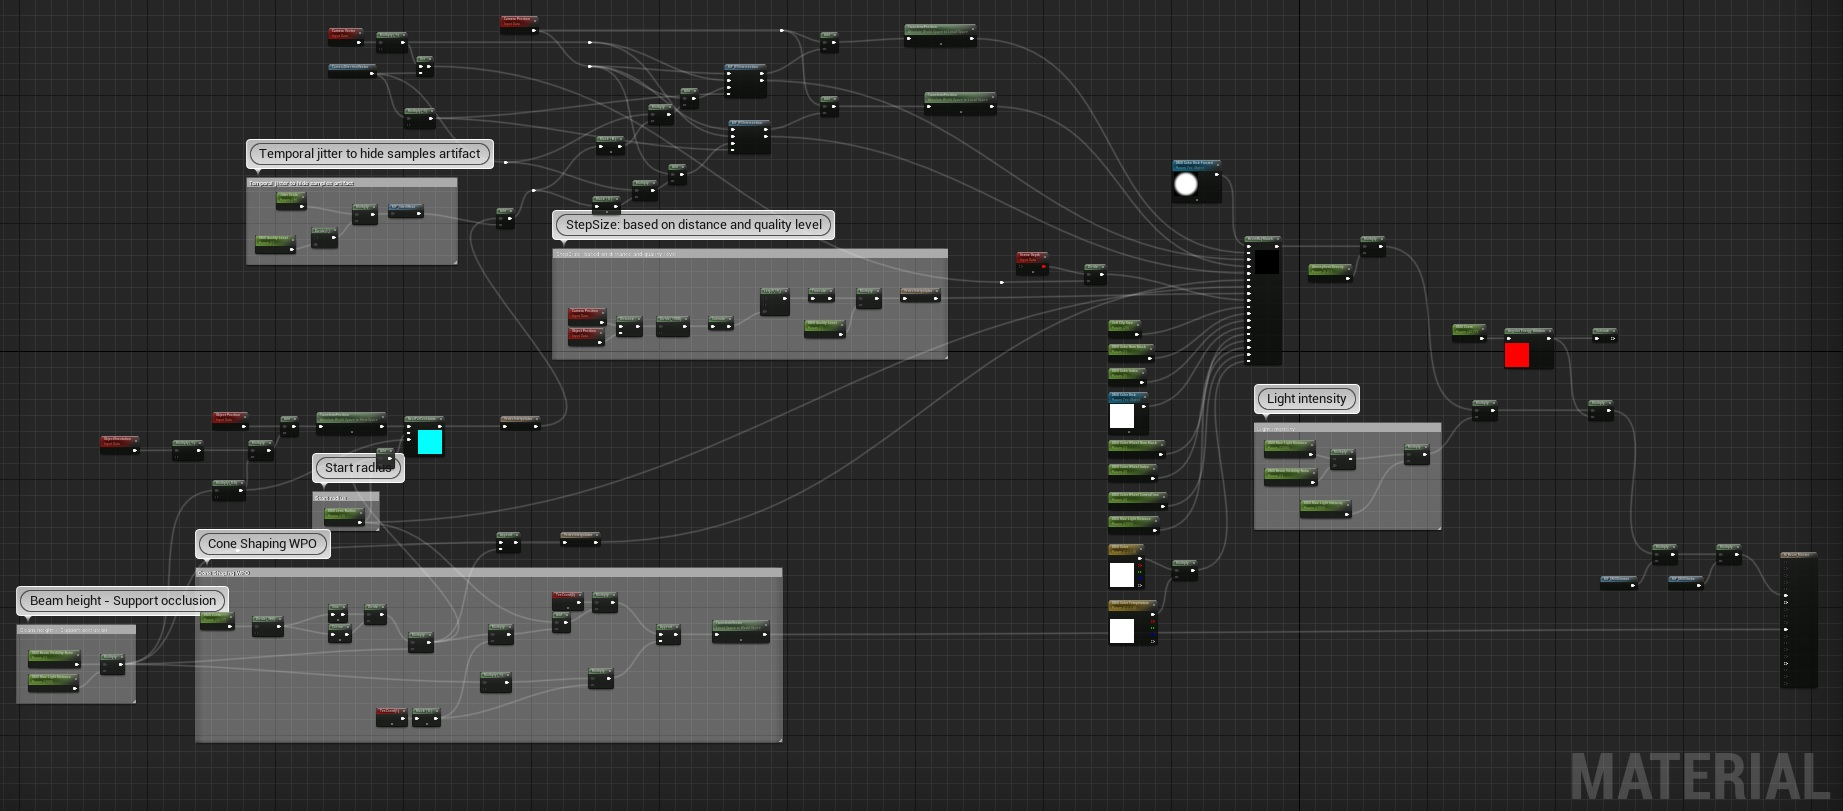
\includegraphics[width=1\linewidth]{img/renderingPipeline/BeamMaterialFull.jpg}
    \caption{Grafo del materiale Beam}
    \label{fig:2_beamGraphFull}
\end{figure}
Per renderizzare un beam, viene utilizzato l'algoritmo \say{Beam RayMarching}. In generale, gli algoritmi di RayMarching \cite{RayMarching} sono degli algoritmi per effettuare il sample di scene tridimensionali che vengono descritte in termini di \textit{SDF}, invece che esplicitamente con geometrie. SDF - \textit{Signed Distance Functions} - sono delle funzioni che ritornano la distanza minima tra un punto ed una superficie e che ci indicano, attraverso il segno, se tale punto si trovi all'interno o all'esterno della superficie stessa.\newline

\begin{wrapfigure}{r}{0.4\textwidth}
    \centering
    \captionsetup{justification=centering}
    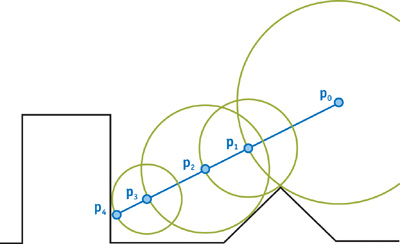
\includegraphics[scale=0.65]{img/renderingPipeline/spheretrace.jpg}
    \caption{Funzionamento dell'algoritmo di RayMarching}
    \label{fig:2_raymarchWikipedia} %taken from https://jamie-wong.com/2016/07/15/ray-marching-signed-distance-functions/
\end{wrapfigure}
Il Raymarching funziona lanciando, a partire dalla camera, un fotone per ogni pixel che deve renderizzare. Questo fotone, nell'implementazione standard, viene mosso iterativamente per un numero di step, fino a colpire un oggetto oppure fino alla fine delle iterazioni. La distanza percorsa ad ogni iterazione è uguale all'SDF tra la posizione del fotone all'iterazione precedente e la superfice della scena, in modo da essere sicuri di non registrare troppo tardi eventuali intersezioni.\newline

Il RayMarching viene spesso usato per generare geometrie che si ripetono, ed è esattamente come viene usato all'interno di questo materiale: per disegnare un beam viene effettuata una operazione di sample più volte, a distanze regolari, della forma della luce che vogliamo proiettare lungo i raggi che escono da una fixture. La distanza tra un sample e l'altro (così come il numero di sample), a differenza da una implementazione pura di Raymarching, varia in base alla distanza dalla telecamera e dalla qualità di rendering scelta. Più sample faremo e più la luce risulterà uniforme. 
\begin{figure}[H]
    \centering
    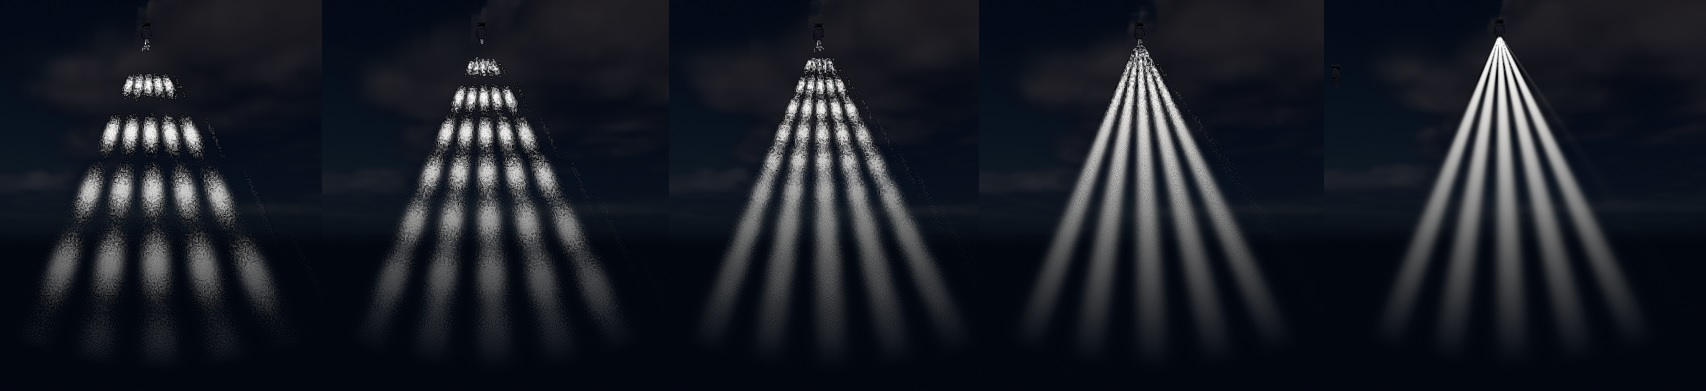
\includegraphics[width=1\linewidth]{img/renderingPipeline/renderingQuality.jpg}
    \caption{Diminuendo o aumentando il numero di sample si vede chiaramente come l'effetto beam sia ottenuto ripetendo la texture che vogliamo proiettare (4 punti in fila orizzontale) un numero elevato di volte.}
    \label{fig:2_raymarchQualities}
\end{figure}

Gran parte del grafo del materiale si occupa della preparazione dei parametri del RayMarching, quali la \lstinline{StepSize} (influenzata dalla qualità di rendering e dalla lontananza del beam), il punto di intersezione con il beam di una luce più vicino e quello più lontano (\lstinline{NSlice} e \lstinline{FSlice}), la distanza da questi punti (\lstinline{NDepth} e \lstinline{FDepth}), la distanza tra la camera e la fine del mondo (\lstinline{SCdepth}), la grandezza della base del beam (\lstinline{ConeRadius}), la distanza che un beam può percorrere e il suo zoom (\lstinline{AdjOpp}), la trasparenza del beam rispetto agli altri oggetti (\lstinline{SoftClipSize}). L'algoritmo effettivo si trova all'interno di una CustomExpression che prende come argomenti, oltre ai parametri calcolati dal grafo, le texture delle ruote gobo e colori (\lstinline{TXTpGobo} e \lstinline{TXTpColor}), la loro grandezza in slot (\lstinline{NumGobos} e \lstinline{NumColors}) e gli indici all'interno delle ruote (\lstinline{GoboIndex} e \lstinline{ColorIndex}). \newline

Inizialmente il codice della CustomExpression si calcola la distanza totale che il nostro fotone percorrerà (\lstinline{traversalDepth}) e, utilizzando StepSize, calcolerà il numero di step che impiegherà a percorrerla (\lstinline{numSteps}) e lo scostamento ad ogni step (\lstinline{posOffset}). Successivamente prenderà la distanza massima (che corrisponde alla potenza in base allo zoom) che può percorrere la luce del faro (\lstinline{Adj}) e il suo zoom (\lstinline{Opp}).
\lstset{language=glsl}
\begin{lstlisting}
float traversalDepth = FDepth - NDepth;
uint numSteps = floor(traversalDepth / StepSize);
float3 posOffset = normalize(FSlice-NSlice) * StepSize;

float Adj = AdjOpp.x;
float Opp = AdjOpp.y + ConeRadius;
\end{lstlisting}

Da qui in poi inizia il loop dell'algoritmo di Beam RayMarching. Il ciclo in se si occupa principalmente di replicare, ad ogni iterazione, la texture che si vuole proiettare, a distanza \lstinline{StepSize} l'una dall'altra. Inoltre, all'interno ha anche il compito di gestire la trasparenza e l'overlay di oggetti posti davanti al fascio di luce. Il ciclo inizia dichiarando una variabile (\lstinline{cumul}) che verrà usata per salvare tutti i vari sample che vengono effettuati ad ogni iterazione, e che poi sarà l'output del RayMarch.
\begin{lstlisting}
float3 cumul = 0;
for(uint i=0; i<numSteps; i++){
    ...
}
return cumul ;
\end{lstlisting}

La prima operazione effettuata nel ciclo è ottenere la distanza e la posizione relativa all'iterazione corrente.
\begin{lstlisting}
///Position & depth at rayHit
float3 pos = NSlice + posOffset * i ;
float depth = NDepth + StepSize * i ;
\end{lstlisting}
Successivamente la posizione viene convertita per essere nel range [0, 1], in modo da poter effettuare sucessivamente le operazioni di sample. A questo punto la nostra posizione è stata convertita in coordinate UV.
\begin{lstlisting}
///Domain Transform
pos.z = -pos.z;
pos /= float3(Opp*2,Opp*2,Adj);

float div = ConeRadius / Opp;
div = (pos.z*(1-div))+div;
pos.xy /= div;

//Center domain
pos.z -= 0.5 ;
\end{lstlisting}
Poi viene verificato che non stiamo disegnando texture dalla parte opposta della fixture, e che non abbiamo un qualche altro oggetto a coprire completamente il beam. Se è valida una delle due condizioni, saltiamo questa iterazione del ciclo.
\begin{lstlisting}
///Clip domain edges.
bool maskX = abs(pos.x) > 0.5;
bool maskY = abs(pos.y) > 0.5;
bool maskZ = abs(pos.z) > 0.5;
if (maskX || maskY || maskZ) continue;

///Soft clipping with scene depth.
float dClip = saturate((ScDepth-depth)/SoftClipSize);
if(dClip == 0) continue;
\end{lstlisting}
A questo punto avviene l'effettivo sample della ruota gobo e colori. Viene prima calcolato l'offset all'interno nella ruota, viene poi usato per modificare la coordinata $X$ delle UV ed infine viene effettuata l'operazione di sampling della texture
\begin{lstlisting}
// UVs from pos
pos.xy = saturate(pos.xy+0.5);

//gobo
float2 texCoor = pos.xy;
float scale = 1 / NumGobos;
float offset = GoboIndex / NumGobos;
texCoor.x = texCoor.x * scale + offset;
float GoboSample = TXTpGobo.SampleLevel(TXTpGoboSampler, texCoor, 0);

//color
ColorUV.x = ColorUV.x / NumColors;
ColorUV.x = ColorUV.x  + (ColorIndex/NumColors) ;
float3 ColorSample =
    TXTpColor.SampleLevel(TXTpColorSampler, ColorUV.xy,0);
// Add DMXColor in
ColorSample = ColorSample * DMXColor;
\end{lstlisting}
\begin{figure}[H]
    \centering
    
\includegraphics[width=1\linewidth]{img/renderingPipeline/Wheel_Rotating_Gobo_Wheel.jpg}
    \caption{Esempio della texture di una ruota gobo. Il motivo per cui viene modificata la coordinata X delle UV è perché la texture di una ruota gobo consiste nelle texture dei singoli slot posti orizzontalmente l'uno accanto all'altro. Modificando la coordinata X si fa scorrere una "finestra" di output quadrata lungo la texture}
    \label{fig:2_goboWheel}
\end{figure}
Infine viene calcolato il valore di decadenza della luce e vengono combinati insieme tutti i valori calcolati fin'ora.
\begin{lstlisting}
float dist = length(pos);
float falloff = 1.0f-(dist/MaxDistance);
// InvSqr falloff function
float invsqr = 1.0f / (dist*dist);

///Add to Result
cumul +=
    (1/numSteps) * GoboSample * ColorSample * dClip * invsqr * falloff;
\end{lstlisting}

Nell'implementazione attuale non esiste la possibilità di implementare più ruote dello stesso tipo: lo evinciamo semplicemente dal fatto che gli input della CustomExpression sono solo uno per tipo di ruota. Inoltre notiamo come nel codice il sampling della ruota colore e di quella gobo viene essenzialmente fatto allo stesso modo, eppure non è stata creata una funzione generalizzata per farlo, bensì due codici specifici per ciascuna. 

\subsubsection{Light}\label{subsec:2_1_light}
Questo materiale si occupa della proiezione della luce su altri materiali
\begin{figure}[H]
    \centering
    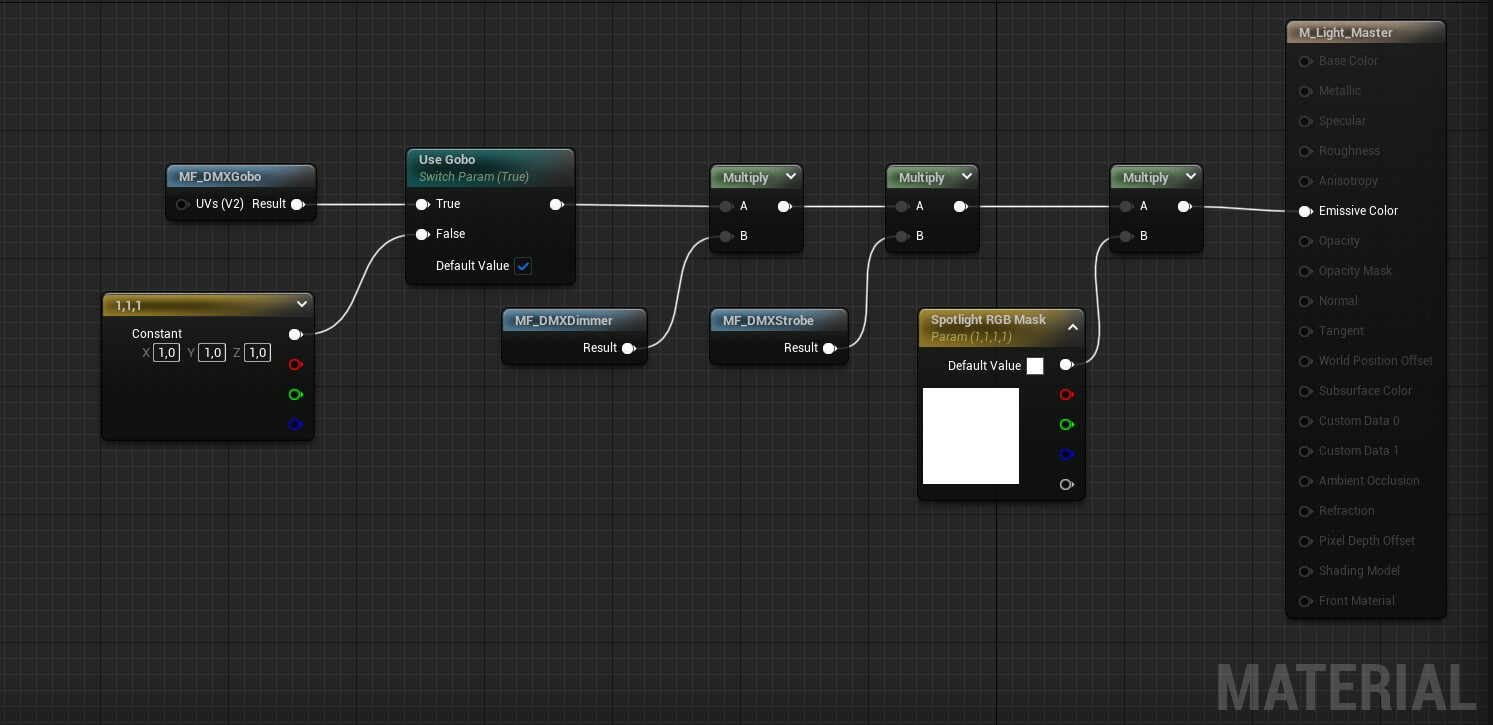
\includegraphics[width=1\linewidth]{img/renderingPipeline/LightMaterialFull.jpg}
    \caption{Grafo del materiale Light}
    \label{fig:2_lightGraphFull}
\end{figure}
Come possiamo notare è molto basilare, abbiamo due MaterialFunctionCall che si occupano dell'elaborazione del dimmer e della strobo, che vengono moltiplicati con il risultato di una terza MaterialFunctionCall chiamata \say{DMXGobo}. Aprendo quest'ultima possiamo notare un grafo più interessante, che è quello con cui vengono renderizzate le ruote.
\begin{figure}[H]
    \centering
    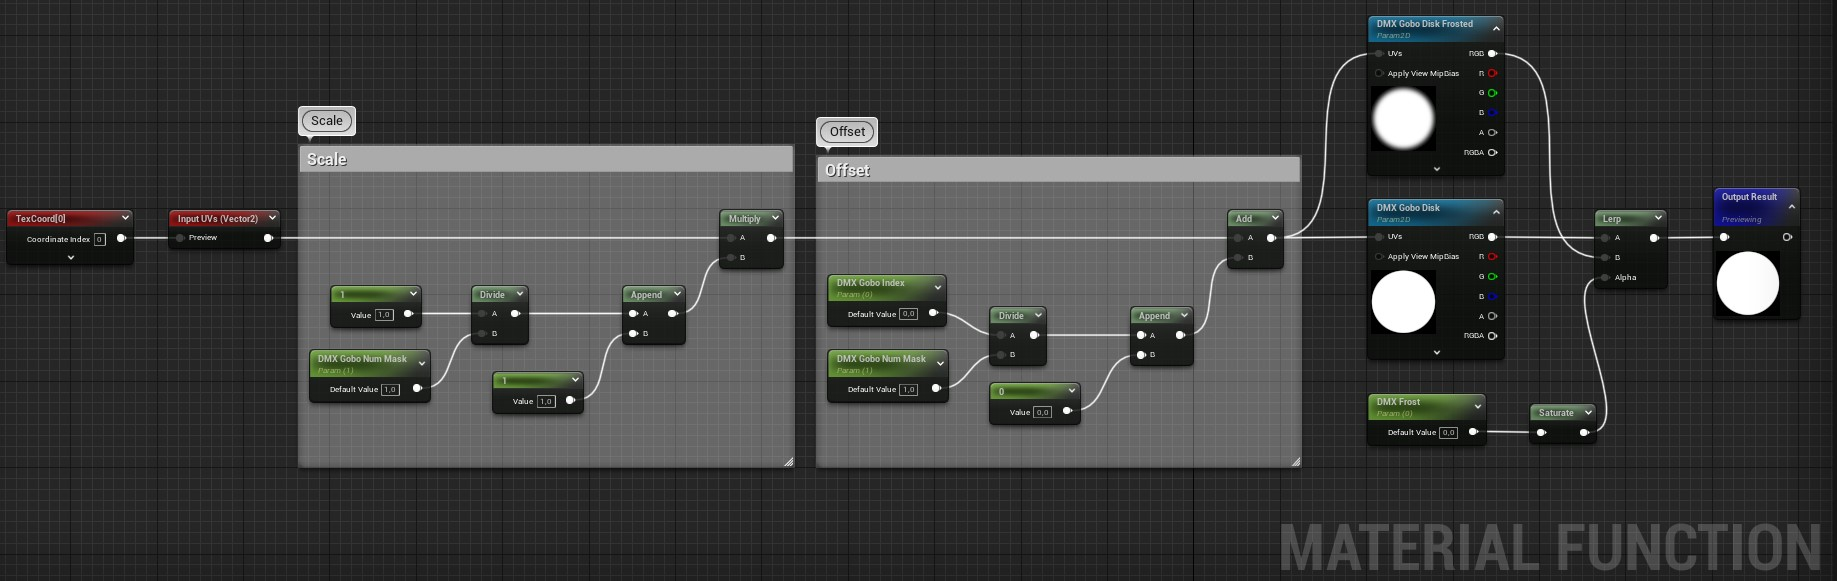
\includegraphics[width=1\linewidth]{img/renderingPipeline/DMXGoboMFFull.jpg}
    \caption{Grafo della Material Function DMXGobo}
    \label{fig:2_dmxGoboGraphFull}
\end{figure}
A sinistra riceviamo in input le coordinate UV che la camera sta renderizzando in quel momento. Successivamente passiamo in due blocchi, che svolgono l'operazione $UV.x * (1 / GoboNumMask) + (GoboIndex / GoboNumMask)$. Notiamo come questo calcolo sia lo stesso utilizzato per fare il sample delle gobo dentro il materiale Beam (\ref{subsec:2_1_beam}). Infatti il risultato viene poi utilizzato come input per due nodi (\say{DMX Gobo Disk} e \say{DMX Gobo Disk Frosted}, uno contiene la texture originale, l'altro una versione sfocata della stessa texture) per effettuare il sample della ruota gobo. Successivamente i due sample vengono interpolati in base al valore del frost (sfocatura) ed infine viene restituito in output.

Da notare come il nome dei parametri all'interno di questa MaterialFunction facciano riferimento solo alle ruote gobo, e come all'interno del Materiale originale sia presente solamente una MaterialFunctionCall a DMXGobo. Questo implica l'impossibilità di renderizzare sia ruote differenti da quelle gobo e l'impossibilità di avere più ruote gobo nella stessa fixture

\subsubsection{Lens}\label{subsec:2_1_lens}
\begin{figure}[H]
    \centering
    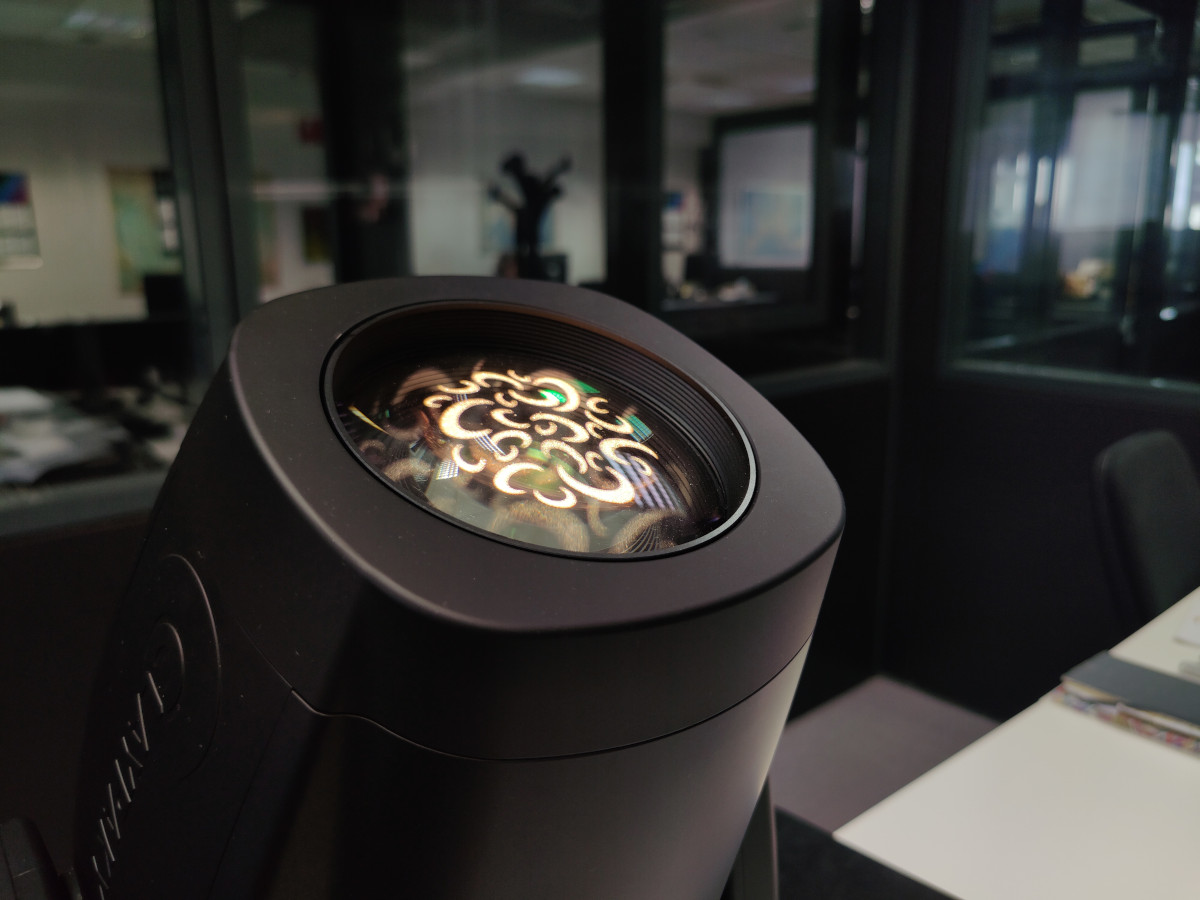
\includegraphics[width=0.5\linewidth]{img/renderingPipeline/Lens.jpg}
    \label{fig:2_Lens}
\end{figure}
Questo materiale si occupa di applicare l'effetto che stiamo renderizzando sulle lenti (virtuali) di un faro
\begin{figure}[H]
    \centering
    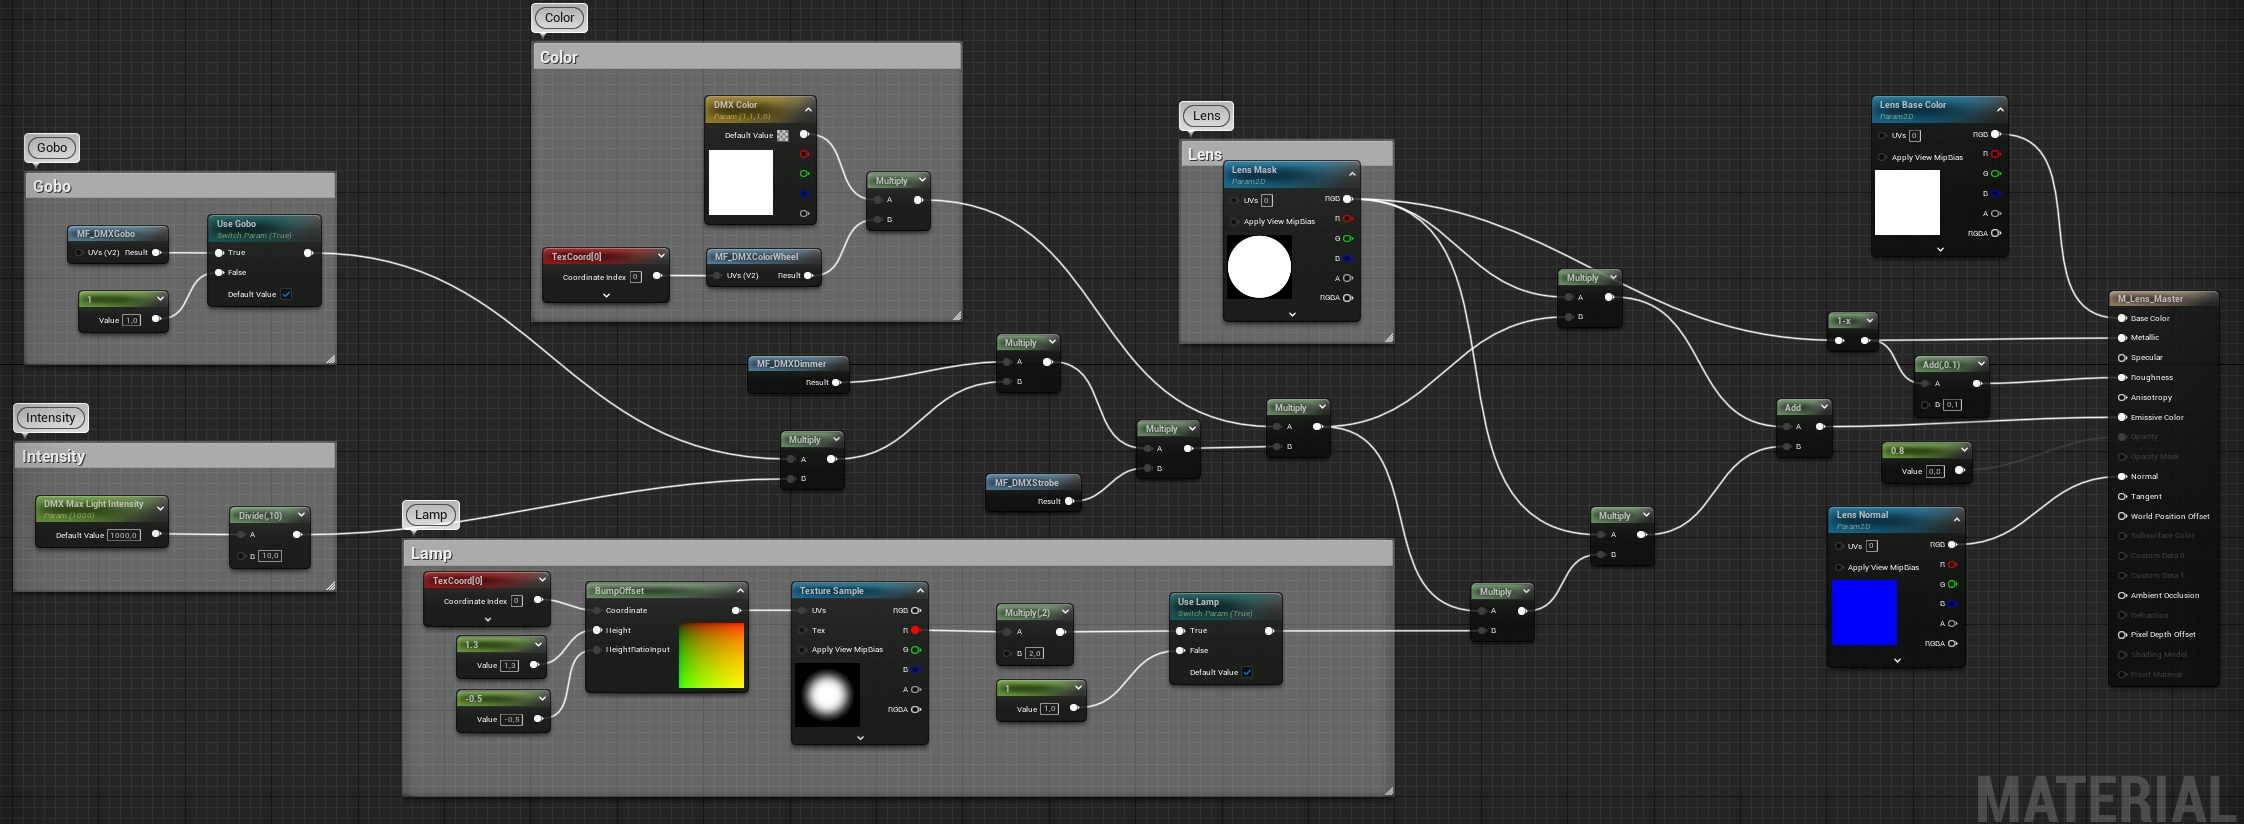
\includegraphics[width=1\linewidth]{img/renderingPipeline/LensMaterialFull.jpg}
    \caption{Grafo del materiale Lens}
    \label{fig:2_lensGraphFull}
\end{figure}
Il grafo è in realtà molto simile a quello visto precedentemente per il materiale Light (\ref{subsec:2_1_light}). Si aggiungono solamente dei blocchi di nodi in più (\say{Lens}, \say{Lamp}) che servono a redere più fotorealistica la resa delle lenti. Anche in questo materiale è presente una MaterialFunctionCall a DMXGobo, ma notiamo come ce n'è un'altra a DMXColorWheel (la quale implementazione è identica a quella delle gobo, nonostante, di fatto, stiano facendo la stessa cosa).

\subsection{Idea della pipeline}\label{subsec:2_pipelineIdea}
Nelle precedenti sezioni abbiamo potuto vedere come allo stato attuale sia davvero difficile aggiungere nuove features e sia impossibile la presenza di più attributi contemporaneamente. Una buona idea per risolvere questi problemi è quella di astrarre il rendering dei vari moduli in moduli generici e realizzare una pipeline il più simile possibile ad una vera fixutre. Come spiegato nell'introduzione (\ref{subsec:1_1_modules}), in una vera luce è presente un emettitore che genera un fascio di luce che attraverserà ogni singolo modulo montato. Ogni modulo prende quindi il \say{risultato} del modulo precedente, ci applica un filtro sottrattivo sopra e lo da in output al modulo successivo. \newline

La stessa identica cosa è stata quindi implementata su Unreal Engine. Verrà creata una nuova MaterialFunction contenente l'intera pipeline. Tutte le feature di una luce vengono trasformate in MaterialFunction che prenderanno in input, oltre ai loro parametri, il valore elaborato dalla precedente MF, e che daranno in output il valore modificato dalla feature. Tutte le feature che riguardano i colori (eccezion fatta della color wheel) verranno renderizzate al di fuori di questa catena di moduli (L'argomento verrà approfondito nel capitolo \ref{sec:FixtureComponentHierachy}) e l'output di questo processo verrà utilizzato come primo nodo della pipeline. L'output dell'ultimo nodo verrà collegato all'output della MaterialFunction. Ogni modulo della pipeline si occuperà, internamente, di fare il rendering della feature, invertirlo matematicamente, e poi sottrarlo al valore del nodo precedente. \newline
Questa MaterialFunction contenente la nuova pipeline verrà quindi piazzata al posto di quella che calcola le ruote gobo dentro il rendering Light e Lens (In quest'ultima verrà rimossa quella che renderizza le ruote colori), in modo da toccare il meno possibile i materiali originali. Nel contesto del materiale originale, è come se stessimo renderizzando una gobo molto elaborata e già colorata. \newline
E per il rendering del Beam?

\subsubsection{Problemi con le MaterialExpressionCustom e le MaterialFunction}\label{subsec:2_2_CM-MFproblems}
Come spiegato nella sezione \ref{subsec:2_1_beam}, il rendering del Beam di luce viene effettuato con una funzione di Raymarching scritta in HLSL dentro una CustomExpression. Purtroppo Unreal Engine non mette a disposizione un modo \say{pulito} per eseguire una MaterialFunction all'interno del codice di una CustomExpression \cite{customExpressionMaterialFunction}. L'unica scelta rimane quindi di riscrivere l'implementazione dei vari moduli come funzioni in hlsl. Possiamo però dichiarare una funzione nel codice di una MaterialExpressionCustom? La risposta è no.
\begin{figure}[H]
    \centering
    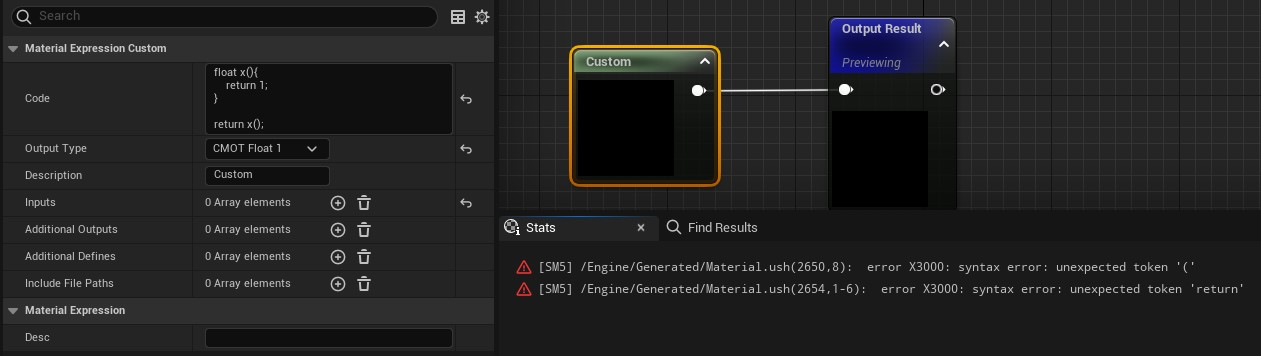
\includegraphics[width=1\linewidth]{img/renderingPipeline/meCustomNoFunc.jpg}
    \caption{Compilare una funzione dentro una CustomExpression ci darà errore}
    \label{fig:2_funcCompileError}
\end{figure}

Unreal Engine ci mette a disposizione tra i suoi vari menù, una finestra per consultare il codice HLSL che viene generato a partire da un Material. Andando a cercare ciò che abbiamo scritto nella MaterialExpressionCustom, notiamo che viene inserito all'interno di un'altra funzione.
\begin{figure}[H] % TODO check that this image always fit inside the page!
    \centering
    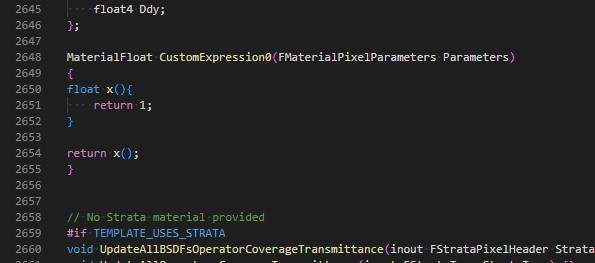
\includegraphics[width=0.8\linewidth]{img/renderingPipeline/hlslFunInUn.jpg}
    \label{fig:2_funcInFunc}
\end{figure}

In C non si può dichiarare una funzione direttamente all'interno di un'altra funzione, è per questo che non compila. Un modo per farlo però è quello di creare ed allocare una struct contenente all'interno le funzioni che vogliamo dichiarare. Utilizzando l'oggetto allocato è poi possibile andare effettivamente a chiamare le funzioni.
\begin{lstlisting}
struct Helper {
    float x(){
        return 1;
    }
};
Helper h;
return h.x();
\end{lstlisting}
Come ci aspettavamo, questo metodo compila con successo. Possiamo quindi implementare i vari moduli come funzioni di una struct di Helper e poi richiamarli durante il loop del raymarching.

Il motivo per cui si sta preferendo mantenere una doppia implementazione dei vari moduli (Sia come materiali che come codice HLSL) deriva dal fatto che quando Unreal Engine va a compilare i materiali in codice HLSL effettua una prima, grossa, ottimizzazione in cui eventuali valori e calcoli che non cambiano durante il rendering di un materiale vengono automaticamente messi in una cache. La stessa cosa non accade al codice HLSL dentro le MaterialExpressionCustom, che viene invece incapsulato senza essere toccato all'interno di una funzione, nel sorgente HLSL del materiale di cui fa parte. \cite{hlslNoOptimize}

\lstset{language=UEcpp}
\subsection{Generazione dinamica del codice e delle MaterialExpression}\label{subsec:2_codeGeneration}
Non tutte fixture hanno gli stessi moduli. Alcune, ad esempio, potrebbero avere il sagomatore, mentre altre no. Inoltre alcune luci possono avere un numero variabile di una stessa feature. Per far fronte a queste differenze, al posto di usare un unico materiale in ogni tipo di fixture, si è scelto di generare programmaticamente una pipeline di rendering per ogni tipo di faro importato. Purtroppo, per poter usare una MaterialFunction (E quindi una pipeline) specifica per ogni attore (rappresentante un tipo di fixture) che viene creato, bisogna che quell'attore abbia anche i propri componenti. Ad ogni import quindi viene prima generata la pipeline, successivamente vengono clonati i materiali Light, Beam e Lens, poi viene inserita una MaterialFunctionCall alla pipeline (o inserito il codice HLSL) nei materiali, ed infine vengono assegnati questi nuovi materiali all'attore. 
Poiché modalità differenti di una fixture possono avere feature (ed in realtà anche geometrie) differenti, questa operazione va fatta per ciascuna modalità e dovranno essere salvate tutte le pipeline e tutti i materiali separatamente.

Viene quindi creata una classe \lstinline{CPGDTFRenderPipelineBuilder} il quale costruttore si occuperà di analizzare i componenti in input per individuare quali e quante features dovranno essere inserite all'interno della pipeline
\begin{lstlisting}
void CPGDTFRenderPipelineBuilder(
        UCPGDTFDescription* gdtfDescription,
        int selectedMode,
        TArray<UActorComponent*> components,
        FString fixturePathOnContentBrowser) {

    //Salva l'indice della modalita' selezionata
	this->mSelectedMode = selectedMode;
	this->mGdtfDescription = gdtfDescription;
	//Ottieni l'array con le ruote presenti in un faro
    this->mWheels = Cast<UDMXImportGDTFWheels>(
        gdtfDescription->Wheels)->Wheels;
    //Salva il nome (sanitizzato) del tipo di fixture
	this->mSanitizedName = UPackageTools::SanitizePackageName(
        Cast<UDMXImportGDTFFixtureType(
            gdtfDescription->FixtureType)->Name.ToString());

    //Genera e salva il path in cui verranno
    //salvati i materiali clonati e la pipeline
	if (fixturePathOnContentBrowser.EndsWith(TEXT("/")))
        fixturePathOnContentBrowser.RemoveAt(
            fixturePathOnContentBrowser.Len() - 1);
	fixturePathOnContentBrowser.Append("/lightRenderingPipeline/");
	fixturePathOnContentBrowser.Append(FString::FromInt(selectedMode));
	fixturePathOnContentBrowser.Append(TEXT("/"));
	this->mBasePackagePath = fixturePathOnContentBrowser;

    //Analizza le ruote del faro e conta quante ce ne sono per tipo
	for (FDMXImportGDTFWheel wheel : this->mWheels) {
		FCPGDTFWheelImporter::WheelType wType =
            FCPGDTFWheelImporter::GetWheelType(
                this->mGdtfDescription,
                wheel.Name,
                selectedMode);
		this->mWheelsNo[wType]++;
	}

    //Analizza gli altri componenti
	for (int i = 0; i < components.Num(); i++) {}
}
\end{lstlisting}

Successivamente viene creato un metodo \lstinline{cloneMaterialInterface()} per creare una copia dei materiali a partire da una sorgente specificata. Questo metodo verrà usato per clonare tutti e 3 i materiali. La generazione della pipeline in se avviene in maniera differente tra beam e light/lens, per questo motivo in input la funzione riceverà una lambda che verrà eseguita una volta che il nuovo materiale è pronto per l'aggiunta di nuovi. Per le operazioni di clone in se utilizziamo la funzione \lstinline{UMaterialExpression::CopyMaterialExpressions()} \cite{CopyMaterialExpressions}, che clona tutti i nodi ed i collegamenti tra un materiale e l'altro senza però copiare il collegamento verso gli output di un materiale. Per ricreare anche quest'ultimo collegamento, la nostra funzione prenderà in input una seconda lambda che si occuperà di cercare gli ultimi nodi del grafo del materiale e di linkarli ai rispettivi output originali.
%    materialType = TEXT("_") + materialType;
%    FString mName = getMaterialFilename(materialType, false);
%
%    UPackage* materialPackage =
%        CreatePackage(*(this->mBasePackagePath + mName));
%    auto materialFactory = NewObject<UMaterialFactoryNew>();
%    UMaterial* dstMaterial =
%        (UMaterial*)materialFactory->FactoryCreateNew(
%            UMaterial::StaticClass(),
%            materialPackage,
%            *mName,
%            RF_Standalone | RF_Public,
%            NULL, GWarn);
%    UMaterialEditorOnlyData* dstMaterialData =
%        dstMaterial->GetEditorOnlyData();
%
%    FString masterMaterialPath = FCPGDTFImporterUtils::BASEPATH;
%    masterMaterialPath = masterMaterialPath
%                       + TEXT("MaterialInstances/Master/M")
%                       + materialType + TEXT("_Master.M")
%                       + materialType + TEXT("_Master");
%    UMaterial* srcMaterial = Cast<UMaterial>(
%        FCPGDTFImporterUtils::LoadObjectByPath(masterMaterialPath));
        
\begin{lstlisting}
bool cloneMaterialInterface(
    FString materialType, //Nome del tipo di materiale
    const std::function<bool(
        UMaterial*,
        UMaterialEditorOnlyData*,
        TArray<TObjectPtr<UMaterialExpression>>
    )>& linkOutputFnc, //Lambda per collegare i nodi all'output
    const std::function<bool(
        UMaterial*,
        UMaterialEditorOnlyData*,
        TArray<TObjectPtr<UMaterialExpression>>
    )>& middleCode) { //Lambda per la generazione/link della pipeline

    //Creazione del materiale di destinazione
    UMaterial* dstMaterial = [...]
    //Caricamento del materiale sorgente
    UMaterial* srcMaterial = [...]

    //Copia dei nodi da un materiale all'altro
	TArray<TObjectPtr<UMaterialExpression>> dstExpression;
	TArray<TObjectPtr<UMaterialExpression>> srcExpression =
        srcMaterial->GetEditorOnlyData()->
        ExpressionCollection.Expressions;
	UMaterialExpression::CopyMaterialExpressions(
        srcExpression, nullptr,
        dstMaterial, nullptr,
        dstExpression, nullptr);
	//Esegui la lambda per collegare gli output del materiale
	if(linkOutputFnc)
        linkOutputFnc(dstMaterial, dstMaterialData, dstExpression);
	//Copia delle proprieta' del materiale
	copyUMaterialDetails(dstMaterial, srcMaterial);

	//Esegui la lambda per generare/inserire la pipeline di rendering
	if(middleCode)
        middleCode(dstMaterial, dstMaterialData, dstExpression);
}
\end{lstlisting}
\clearpage % TODO check if we really need this
\begin{wrapfigure}{r}{0.4\textwidth}
    \centering
    \captionsetup{justification=centering}
    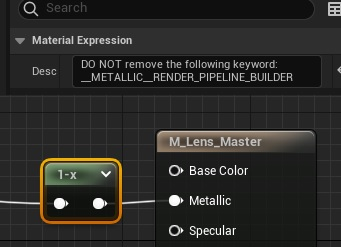
\includegraphics[scale=0.65]{img/renderingPipeline/descLink.jpg}
    \caption{Esempio di descrizione dentro il nodo che si collega all'out}
    \label{fig:2_searchDesc}
\end{wrapfigure}
Unreal Engine permette di impostare una descrizione o commento per ogni nodo. Questa descrizione verrà usata per trovare i nodi da collegare agli output dei materiali o da collegare alla pipeline di rendering, poiché ci serve un modo deterministico per ottenere sempre i nodi corretti. Viene quindi inserito un identificativo nella descrizione di ogni nodo che deve essere collegato in output o alla pipeline e verrà creata una funzione templatizzata per ricercare un nodo di un determinato tipo con un determinato identificativo all'interno di un materiale:
\begin{lstlisting}
template <typename CheckType>
CheckType* searchMaterialExpressionByDesc(
        //Lista di nodi in un materiale
        TArray<TObjectPtr<UMaterialExpression>> arr,
        //Identificativo da cercare
        FString descr) {
    for (TObjectPtr<UMaterialExpression> mePtr : arr) {
        UMaterialExpression* me = mePtr.Get();
        if (me->Desc.Contains(descr)) {
            CheckType* casted = Cast<CheckType>(me);
            //Cast<T>() ritorna null se l'oggetto non e' castabile a T
            if (casted) return casted;
        }
    }
    return nullptr;
}
\end{lstlisting}

Ogni volta che viene creato un nuovo nodo, esso viene inserito a coordinate (0, 0) all'interno del grafo del materiale. Andare ad effettuare del debugging su un materiale in cui sono stati generati tante MaterialExpression può essere pesante per via del disordine che si crea nell'avere tutti i nodi l'uno sull'altro. È nata quindi la necessità di creare una nuova classe di helper specializzata nel posizionare automaticamente i nuovi nodi ad intervalli regolari l'uno dall'altro. 
Questa classe ha bisogno di sapere l'asse sul quale ci stiamo muovendo, le coordinate dell'ultima MaterialExpression spostata, ed lo spiazzamento tra l'una e l'altra. Il costruttore è molto semplice, si prende queste 4 informazioni e se le salva. Il metodo \lstinline{moveMaterialExpression} (Responsabile di muovere i nodi) banalmente imposterà l'x e la y della MaterialExpression in input a quelli correnti, sceglierà una coordinata in base all'asse che stiamo percorrendo e la aggiornerà dell'offset prestabilito (o uno specificato alla funzione).
\clearpage % TODO check if we really need this
\begin{lstlisting}
struct MeBlocksMover {
    private:
    bool movingYAxys = false;
    int32 x, y;
    int32 defaultOffset;

    public:
    MeBlocksMover(int32 x, int32 y, int32 offset, bool movingYAxys) :
        movingYAxys(movingYAxys), x(x), y(y), defaultOffset(offset) {}

    void moveMaterialExpression(UMaterialExpression* me, int offset=0) {
        me->MaterialExpressionEditorX = x;
        me->MaterialExpressionEditorY = y;

        if (offset == 0) offset = defaultOffset;
        if (movingYAxys) y += offset;
            else x += offset;
    }
    void moveMaterialExpressions(TArray <UMaterialExpression*>& mes) {
        for (UMaterialExpression* me : mes)
            moveMaterialExpression(me);
    }

    inline int32 getCurrentX() {
        return x;
    }
    inline int32 getCurrentY() {
        return y;
    }
};
\end{lstlisting}

Infine vengono create una serie di funzioni inline che generano i nomi dei parametri ed il nome delle variabili del codice HLSL in modo da standardizzare la nomenclatura all'interno dell'itero plugin CPGDTF-Importer. Con \lstinline{get*ParamName()} ci riferiamo a funzioni che generano il nome di parametri all'interno di materiali. Invece, con \lstinline{getInput*Name()} ci riferiamo alla generazione dei nomi per le variabili (e, conseguentemente, ai nomi per gli input) della CustomExpression responsabile di implementare la pipeline di rendering per il materiale Beam.

Nelle successive sezioni andremo a vedere come viene effettivamente generata e linkata la pipeline di rendering, separatamente per il materiale Beam e per i materiali Light e Lens (che condividono la stessa pipeline). Viene anche affrontato il problema di come generare nuove MaterialExpressionParameter all'interno di un materiale, attività che comporta una serie di step ripetitivi riassumibili in una funzione. Il materiale Beam differisce nell'aggiunta di nuove MaterialExpressionParameter poiché devono anche essere automaticamente linkate alla CustomExpression responsabile del Raymarching

\subsubsection{Custom Material (per Beam)}\label{subsec:2_3_CM}
Come accennato sopra, generare un nuovo parametro per la pipeline del beam consiste in una serie di operazioni ripetitive:
\begin{itemize}
    \item Generare un nuovo MaterialExpressionParameter
    \item Impostargli informazioni quali nome, gruppo di parametri, priorità, valore default
    \item Aggiungerlo alla lista delle MaterialExpression del materiale a cui lo stiamo aggiungendo
    \item Generare un nuovo input per le CustomExpression
    \item Dargli un nome (Che verrà utilizzato anche come nome della variabile nel codice HLSL)
    \item Connettergli la MaterialExpressionParameter
    \item Aggiungere l'input alla custom expression che contiene il codice HLSL
    \item Riposizionare l'input usando un oggetto \lstinline{MeBlocksMover}
\end{itemize}
Il codice che si occupa di queste operazioni è il seguente:
\begin{lstlisting}
UMaterialExpressionScalarParameter* addScalarInputToBeamPipeline(
        UMaterial* beamMaterial, //Materiale di destinazione
        FString paramName, //Nome del parametro
        FString inputName, //Nome dell'input della CustomExpression
        UMaterialExpressionCustom* meCustom,
        MeBlocksMover* mover = nullptr,
        float defaultValue = 0) {
    UMaterialExpressionScalarParameter* param =
        generateMaterialExpression<UMaterialExpressionScalarParameter>(
        beamMaterial);
    param->ParameterName = FName(*paramName);
    param->Group = FName(TEXT("Runtime Parameters"));
    param->SortPriority = 5;
    param->DefaultValue = defaultValue;
    beamMaterial->GetEditorOnlyData()->
        ExpressionCollection.AddExpression(param);

    FCustomInput input;
    input.InputName = FName(*inputName);
    input.Input.Connect(0, param);
    meCustom->Inputs.Add(input);

    if(mover)
        mover->moveMaterialExpression(param, SCALAR_PARAM_SIZE_Y);
    return param;
}
\end{lstlisting}

Per la generazione del codice HLSL è stata salvata in una costante del precompilatore una versione modificata del codice originale. Innanzitutto ad inizio codice è stata creata una struttura \lstinline{FunctionsWrapper} contenente le varie funzioni che abbiamo bisogno di chiamare durante la generazione. La funzione di sampling delle ruote è stata generalizzata e spostata in questa struttura:
\lstset{language=glsl}
\begin{lstlisting}
float4 sampleWheel(
        Texture2D txt, SamplerState txtSampler, //Dati della texture
        float2 texCoor, //UV, passato via copia
        float nSlots, //Numero di slot nella ruota
        float index){ //Indice nella ruota
    float scale = 1 / nSlots;
    float offset = index / nSlots;
    texCoor.x = texCoor.x * scale + offset;
    return txt.SampleLevel(txtSampler, texCoor, 0);
}
\end{lstlisting}
Al posto del sampling della gobo è stato aggiunto del codice che prende il valore \lstinline{DMXColor} corrente, lo clampa in alto, esegue la pipeline ed infine lo clampa in basso. Al posto della pipeline, nella costante del preprogrammer, è stato inserito un commento (definito come: \lstinline{#define TEMPLATE_PLACEHOLDER "/*__HLSL_GENERATE_PIPELINE__*/"}) che poi, attraverso un'operazione di find e replace, verrà automaticamente sostituito con del vero codice.
\begin{lstlisting}
float3 outputSample = DMXColor;
if(outputSample.x > 1) outputSample.x = 1;
if(outputSample.y > 1) outputSample.y = 1;
if(outputSample.z > 1) outputSample.z = 1;
FunctionsWrapper _fncs; //Struttura per le chiamate a funzione
"TEMPLATE_PLACEHOLDER"
if(outputSample.x < 0) outputSample.x = 0;
if(outputSample.y < 0) outputSample.y = 0;
if(outputSample.z < 0) outputSample.z = 0;
\end{lstlisting}
Infine è stata modificata la funzione per il calcolo del risultato, in modo da usare la variabile \lstinline{outputSample} e rimuovendo \lstinline{DMXColor} poiché già inclusa nella precedente variabile:\newline \lstinline{cumul += (1.f / numSteps) * outputSample * dClip * invsqr * falloff;}\newline


La generazione del codice in se viene fatta attraverso l'uso di varie printf e StringFormat innestate. Vengono utilizzati entrambi i metodi poiché UnrealEngine presenta una discrita incompatibilità tra tipi (Una printf non può prendersi come stringa di formattazione il risultato di un'altra printf). Per evitare di convergere a nero troppo velocemente quando si hanno troppi filtri, il risultato di ciascuno viene prima elevato alla $1/3$.
\clearpage % TODO check if we really need this
\lstset{language=UEcpp}
\begin{lstlisting}
FString generateHLSLCode() {
    FString outputCode = TEXT(BASE_TEMPLATE);
    FString placeholderCode = TEXT("");

    //Separiamo la creazione del template per poterla modificare
    //in maniera piu' semplice
    FString callText = TEXT("_fncs.{0}");
    FString powText = FString::Printf(
            TEXT("pow(%s, 0.66)"),
        *callText);
    //pow(_fncs.{0}, 0.66)
    FString textAdd = FString::Printf(
            TEXT("\toutputSample = outputSample - 1 + %s;\n"),
        *powText);
    //outputSample = outputSample - 1 + pow(_fncs.{0}, 0.66);
    
    FString frostVarName = getInputFrostName();

    //GENERAZIONE EFFETTIVA QUI

    //Inserimento del codice generato nel template
    FString from = TEXT(TEMPLATE_PLACEHOLDER);
	outputCode = outputCode.Replace(
        *from, *placeholderCode, ESearchCase::CaseSensitive);
	return outputCode;
}
\end{lstlisting}

Attualmente, solamente le ruote colori e gobo sono implementate, ma in vista di eventuali aggiunte future scorriamo lo stesso l'enum di tutti i tipi possibili di ruote. Per ciascun tipo poi, andiamo a generare un numero di ruote pari a quanti componenti di quel tipo esistono nella fixture. Se in una luce non è presente alcuna ruota gobo, andiamo comunque ad aggiungere un sample di una ruota contenente un singolo slot aperto, in modo da applicare comunque una texture circolare realistica al beam
\begin{lstlisting}
bool foundGobo = false;

for (int i = 0; i < FCPGDTFWheelImporter::WheelType::SIZE; i++) {
    FCPGDTFWheelImporter::WheelType wheelType = i;
    switch (i) {
    
    case FCPGDTFWheelImporter::WheelType::Color:
    for (int j = 0; j < this->mWheelsNo[i]; j++) {
        FString txtVarName = getInputTextureName(wheelType, false, j);
        FString numSlotVarName = getInputNumSlotsName(wheelType, j);
        FString indexVarName = getInputIndexName(wheelType, j);

        placeholderCode = placeholderCode + FString::Format(*textAdd, {
            FString::Printf(
                TEXT("sampleWheel(%s, %sSampler, pos.xy, %s, %s)"),
            *txtVarName, *txtVarName, *numSlotVarName, *indexVarName)
        });
    }
    break;
    case FCPGDTFWheelImporter::WheelType::Gobo:
    for (int j = 0; j < this->mWheelsNo[i]; j++) {
        FString txtVarName = getInputTextureName(wheelType, true, j);
        FString numSlotVarName = getInputNumSlotsName(wheelType, j);
        FString indexVarName = getInputIndexName(wheelType, j);
        
        placeholderCode = placeholderCode + FString::Format(*textAdd, {
            FString::Printf(
                TEXT("sampleWheel(%s, %sSampler, pos.xy, %s, %s)"),
            *txtVarName, *textureVarName, *txtVarName, *indexVarName)
        });
        foundGobo = true;
    }
    break;
    default:
    break;
    }
}

if (!foundGobo) //Filter the beam shape anyway if there's no gobo
    placeholderCode = placeholderCode +
        TEXT("outputSample *=
        pow(TXTpGobo.SampleLevel(
        TXTpGoboSampler, pos.xy, 0).x, 0.66);");

\end{lstlisting}
Quando in futuro si vorranno fare aggiunte di nuovi tipi di ruota, basterà aggiungerli nel precedente loop. Se invece si vorranno implementare feature totalmente nuove, si potrnano scrivere semplicemente dopo questo codice.\newline

Una volta generato il codice HLSL bisogna inserirlo all'interno della relativa CustomExpression ed aggiungere gli input necessari alla stessa. Per fare ciò andiamo ad utilizzare la funzione \lstinline{cloneMaterialInterface} di cui abbiamo discusso prima. Come prima lambda, quella che si occupa di collegare le material expression all'output, abbiamo un codice molto semplice, che cerca i nodi corretti e li connette:
\begin{lstlisting}
UMaterialExpressionTransform* meWorldPosOffset =
    searchMaterialExpressionByDesc<UMaterialExpressionTransform>(
    dstExpression, FIND_DESCR_WORLDPOSITIONOFFSET);
if (meWorldPositionOffset)
    dstMaterialData->WorldPositionOffset.Connect(0, meWorldPosOffset);

UMaterialExpressionMultiply* meEmissiveColor =
    searchMaterialExpressionByDesc<UMaterialExpressionMultiply>(
    dstExpression, FIND_DESCR_EMISSIVECOLOR);
if (meEmissiveColor)
    dstMaterialData->EmissiveColor.Connect(0, meEmissiveColor);
\end{lstlisting}

Per quanto riguarda invece la seconda lambda, abbiamo un codice un po' più elaborato, poiché si occupa anche di generare gli input per la CustomExpression.
Inizialmente andiamo a cercare la CustomExpression. Se esiste, generiamo il codice HLSL e glielo impostiamo. Successivamente creiamo l'input per il valore di frost e lo piazziamo dentro il materiale un \lstinline{MeBlocksMover}.
\begin{lstlisting}
UMaterialExpressionCustom* meCustom =
    searchMaterialExpressionByDesc<UMaterialExpressionCustom>(
    dstExpression, FIND_DESCR_CUSTOM);
if (meCustom) {
    meCustom->Code = generateHLSLCode();
    
    MeBlocksMover* meBlocksMover =
        new MeBlocksMover(BEAM_STARTING_X, BEAM_STARTING_Y, 0, true);
    UMaterialExpressionScalarParameter* scalarFrost =
        addScalarInputToBeamPipeline(
            dstMaterial,
            getFrostParamName(),
            getInputFrostName(),
            meCustom,
            meBlocksMover
        );
\end{lstlisting}
Carichiamo poi una texture di default che verrà utilizzata in ogni ruota:
\begin{lstlisting}
FString defaultTexturePath = FCPGDTFImporterUtils::BASEPATH;
defaultTexturePath += "MI/Textures/T_Circle_01.T_Circle_01";
UTexture2D* defaultTexture = Cast<UTexture2D>(
    FCPGDTFImporterUtils::LoadObjectByPath(defaultTexturePath)
);
\end{lstlisting}
E infine, per ogni tipo di ruota (saltando quelli non supportati) e per ogni ruota dello stesso tipo, andiamo ad aggiungere alla CustomExpression gli input ed i parametri per la texture, il numero di slot e l'indice:
\begin{lstlisting}
for (int i = 0; i < FCPGDTFWheelImporter::WheelType::SIZE; i++) {
    FCPGDTFWheelImporter::WheelType wheelType = i;
    for (int j = 0; j < this->mWheelsNo[wheelType]; j++) {

        //Salta tipi non supportati
        if (wheelType == FCPGDTFWheelImporter::WheelType::Animation ||
            wheelType == FCPGDTFWheelImporter::WheelType::Prism ||
            wheelType == FCPGDTFWheelImporter::WheelType::Effects
        ) continue;

        //Parametri per l'index/numero di slot
        addScalarInputToBeamPipeline(
            dstMaterial,
            getNumSlotsParamName(wheelType, j),
            getInputNumSlotsName(wheelType, j),
            meCustom, meBlocksMover, 1);
        addScalarInputToBeamPipeline(
            dstMaterial,
            getIndexParamName(wheelType, j),
            getInputIndexName(wheelType, j),
            meCustom, meBlocksMover);

        //Texture parameter
        bool frosted =
            wheelType == FCPGDTFWheelImporter::WheelType::Gobo;
        addTextureInputToBeamPipeline(dstMaterial,
            getDiskParamName(wheelType, frosted, j),
            getInputTextureName(wheelType, frosted, j),
            meCustom, defaultTexture, meBlocksMover);
    }
}
\end{lstlisting}
Come per la generazione del codice HLSL, aggiungere nuove features che non siano ruote alla pipeline è una operazione facile: Basta semplicemente aggiungerne il codice dopo questo for.\newline

Il risultato dell'esecuzione di questo codice a seguito di una importazione è il seguente: 
\begin{wrapfigure}{r}{0.4\textwidth}
    \centering
    \captionsetup{justification=centering}
    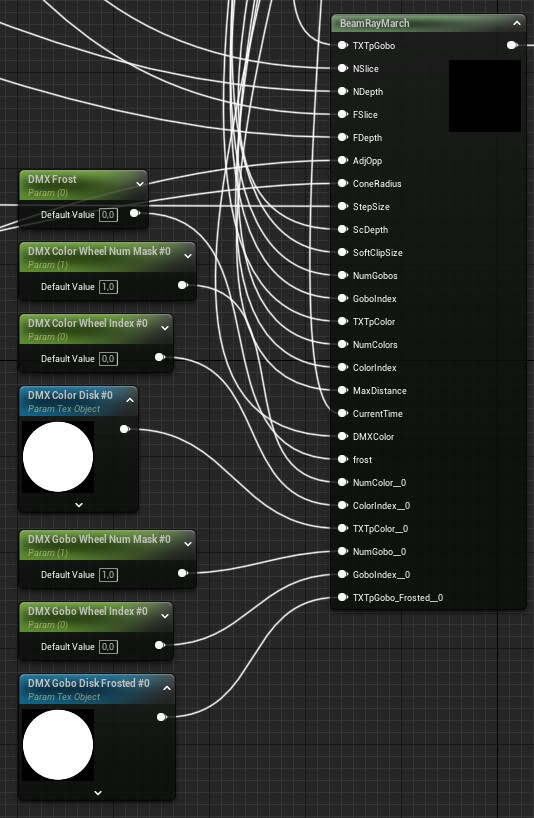
\includegraphics[scale=0.516]{img/renderingPipeline/beamMaterialGenerated.jpg}
    \label{fig:2_beamGenerated}
\end{wrapfigure}
\begin{lstlisting}
float3 outputSample = DMXColor;
if(outputSample.x > 1)outputSample.x = 1;
if(outputSample.y > 1)outputSample.y = 1;
if(outputSample.z > 1)outputSample.z = 1;
FunctionsWrapper _fncs;
outputSample = outputSample - 1 +
    pow(_fncs.sampleWheel(
        TXTpColor__0,
        TXTpColor__0Sampler,
        pos.xy,
        NumColor__0, ColorIndex__0),
    0.66);
outputSample = outputSample - 1 +
    pow(_fncs.sampleWheel(
        TXTpGobo_Frosted__0,
        TXTpGobo_Frosted__0Sampler,
        pos.xy,
        NumGobo__0, GoboIndex__0),
    0.66);
if(outputSample.x < 0)outputSample.x = 0;
if(outputSample.y < 0)outputSample.y = 0;
if(outputSample.z < 0)outputSample.z = 0;
\end{lstlisting}

\subsubsection{Material Function (per Light e Lens)}\label{subsec:2_3_MF}


\end{document}